\documentclass[12pt]{article}
\usepackage{graphicx}

\newcommand{\PF}[1]{\marginpar{\tiny PF: #1}}

\begin{document}

\section{Introduction to FPGAs}

\subsection{How do FPGAs work?}
TO BE COMPLETED ASAP

\subsection{The FPGA design workflow on Quartus}
TO BE COMPLETED ASAP

\subsection{Verilog, a Hardware Description Language}
TO BE COMPLETED ASAP

\section{The DE10-nano board}

\subsection{Intel Cyclone V chip}
The DE10-nano development board is equipped with an FPGA from intel: Cyclone V. This chip is interesting because it not only contains an FPGA but also an ARM processor, it is a FPGA+SoC chip. The advantage of this style of architecture is to have on one side an OS such as linux that runs on a real processor and on the other side the possibility to configure a kind of peripheral on the FPGA side. Moreover, the circuits implemented on the FPGA side can be configured from the ARM processor side, which makes the FPGA part editable in real time. A very interesting example of use is hardware acceleration. One might want to create an audio system on the processor and need different calculation functions: Fourier transform, AC/DC converter, ... All these could simply be implemented by the ARM on the FPGA side whenever needed and use it afterwards if the FPGA space is critical. In the case space is not critical, all the operations can simply be permanently implemented on the FPGA. By doing this, it is often possible to reduce the number of atomic operations required for the complex operation implemented - the operation is now done in hardware and no longer in software.

\subsection{Peripherals}

\begin{figure}[ht!]
  \center
  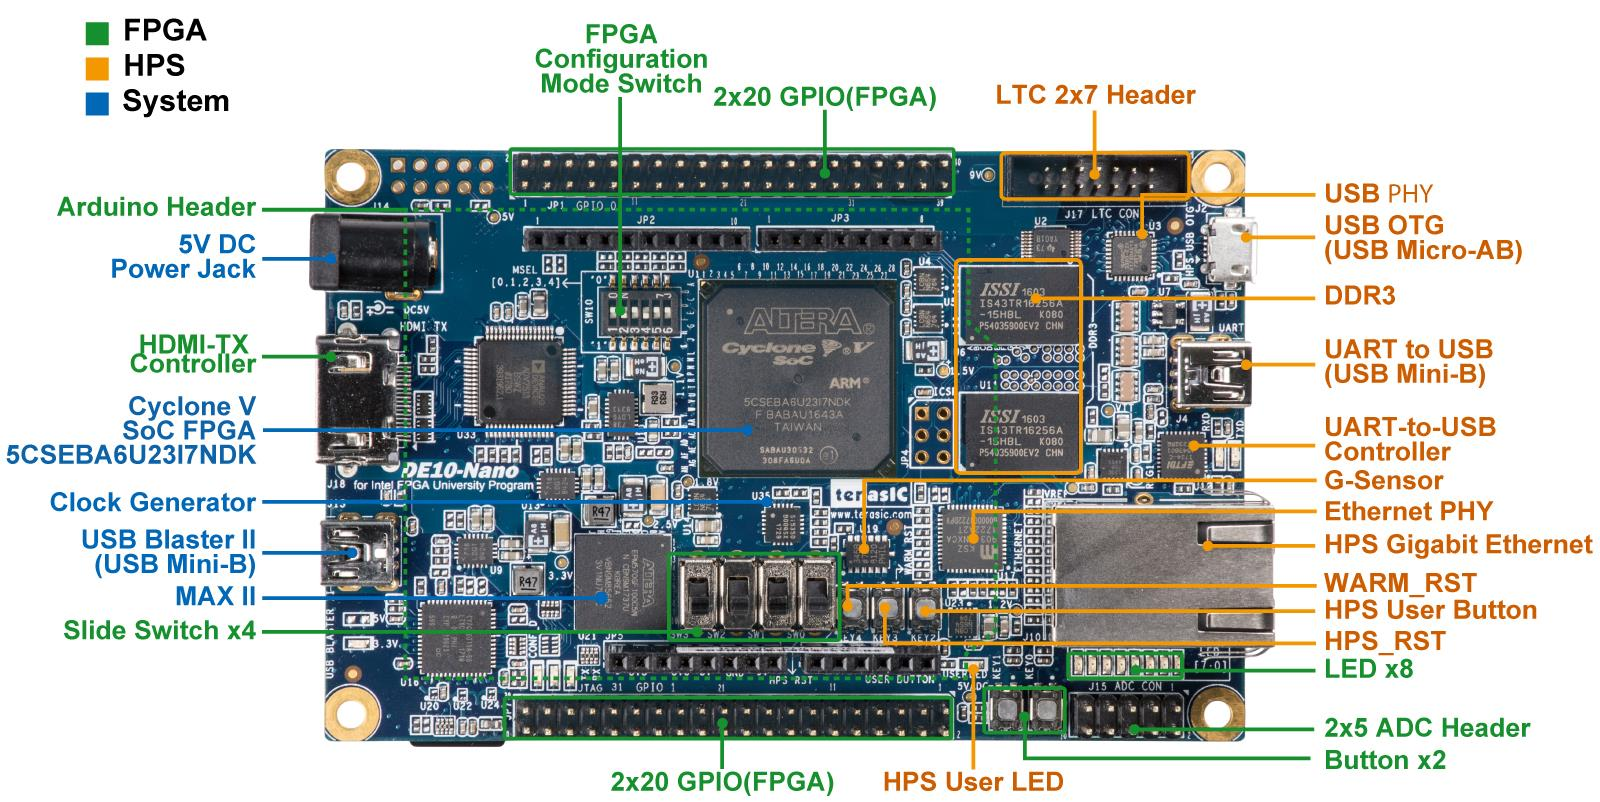
\includegraphics[width=12cm]{"res/chapter1/layout_components.png"}
  \caption{Layout and peripherals of the DE10-nano board}
  \label{fig:de10nano_peripherals}
\end{figure}

On the card, numerous peripherals are made available to the user. Some of them will be very interesting for this work: the DDR3 RAM memory, the SD card reader, the USB controller, as well as the HDMI output. Others allow to make tests, to check the operation without necessarily going through simulation. In this category, there are for example the General Purpose Input / Output pins (GPIOs), LEDs, buttons and sliders. And finally, there are other interesting peripherals that will not necessarily be used in this work such as the Inertial Measurement Unit (IMU) which contains gyroscopes, accelerometers and magnetometers and the ethernet controller.

\vspace{12pt}
All these devices are shown in the Figure \ref{fig:de10nano_peripherals}. It should be noted that the devices are always linked to one of the two parts of Cyclone-V. This means that the other part cannot access them directly. In order to access one of the peripherals on the other side, it will be necessary to use one of the bridges between the ARM part and the FPGA
part.

\subsection{Maximum resource counts}

\subsection{On-chip memory}

\subsection{Connections between ARM and FPGA sides}

The two parts of the architecture can communicate with each other. Indeed, there are several bridges that allow this. First of all, there are those in which the ARM processor is the master: HDS-TO-FPGA bridge and the lightweight HDS-TO-FPGA bridge. Both allow the same operations, except that the lightweight is limited to 32-bit words, while the other allows words up to 128 bits. In the other direction, where the FPGA is the master, there are two bridges again but this time they are more different. The first one is the FPGA-TO-HDS bridge which works like its counterpart, the HDS-TO-FPGA which goes the other way. The second bridge is the FPGA-TO-SDRAM bridge which allows 6 masters on the FPGA side to have direct access to the SDRAM controller. The advantage of the second bridge is that it allows a simple access to the memory but it has the disadvantage of not being cache-coherent with respect to the ARM processor cache. If one wants to have cache-coherency, it is necessary to go through the FPGA-TO-HPS bridge which has the advantage of going through the ARM processor and its cache to access the RAM.

\vspace{12pt}
The different bridges and their points of departure and arrival are described in the diagram in Figure \ref{fig:de10nano_schematic}. The FPGA-TO-SDRAM bridge is not really represented but they are the two wires between the "1 - 6 Masters" block on the FPGA side and the "SDRAM Controller Subsystem" block on the HPS side.

\begin{figure}[ht!]
  \center
  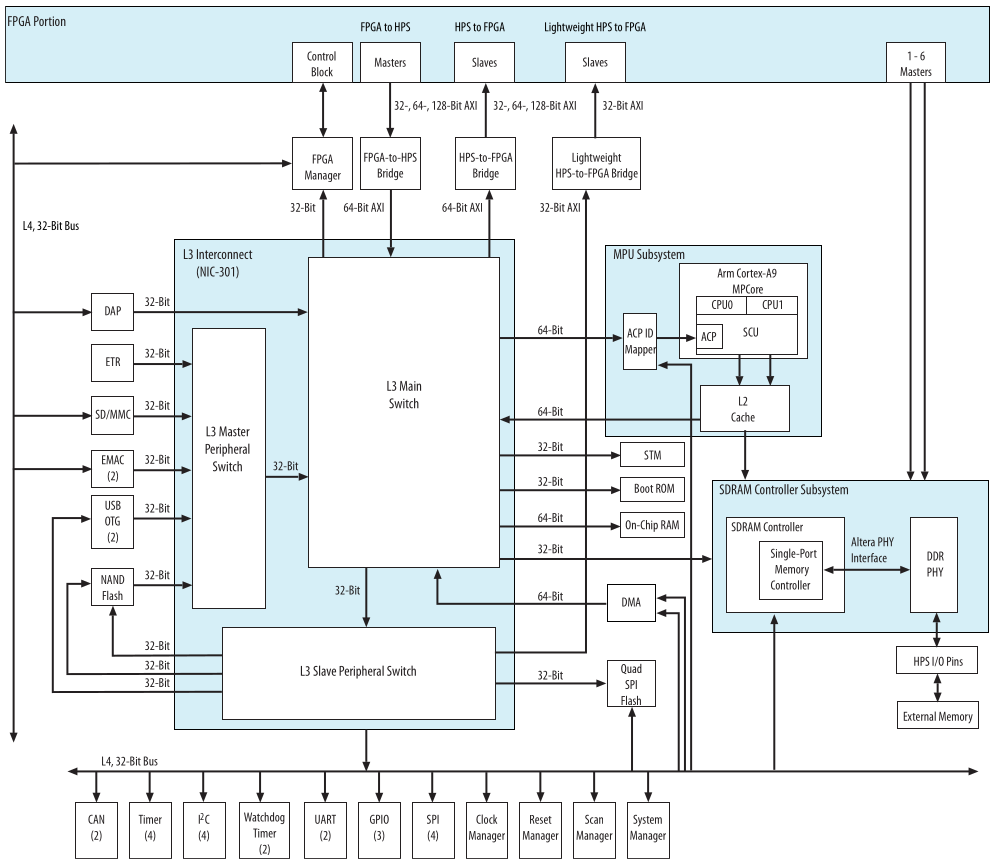
\includegraphics[width=12cm]{"res/chapter1/board_schematic.png"}
  \caption{High level schematic of the DE10-nano board}
  \label{fig:de10nano_schematic}
\end{figure}

\subsection{Communication between ARM and FPGA sides}

The communication between the two parts takes place via one of the above-mentioned bridges using the Avalon protocol described by Intel. This protocol and the interface that goes with it allow high-speed communication. The Avalon interface has different sub-interfaces for different types of communication. Each type is adapted to certain applications. In this project where the protocol will be used to communicate between master(s) and some slave devices, the Avalon MM will be used. The Avalon MM protocol is address based which is very suitable for the needs of this project.

\vspace{12pt}
With this protocol, the idea is quite simple. One is going to write to a certain address or read there. To do this, the protocol detailed below is to be implemented. The protocol allows writing and reading by burst (up to 512 words of 128 bits). It was therefore decided to directly take into account this capability rather than using the simplified version of the protocol that does not include burst.

\subsubsection{Read burst operation}

First, let's start by reading. The sequence diagram of the protocol for the reading operation is visible in Figure \ref{fig:avalon_mm_read}. In the diagram, two masters are represented but only the unique master case will be described. In the first place, the master will simply have to give the start address to which it wants to read, the length of the burst (the number of words desired) as well as to switch the read and beginbursttransfer signals to high. The slave will then respond to this with a waitrequest that will go up. The master must imperatively keep all signals except beginbursttransfer which returns to the low state unchanged during the waitrequest to give the slaves time to capture them. Once ready, the slave will remove the waitrequest and inform that the data is available by switching readdatavalid to high and sending the first word. The other words are then sent to the master in the order of their addresses. As one can see, the bigger the burst, the longer the delay of a read.

\begin{figure}[ht!]
  \center
  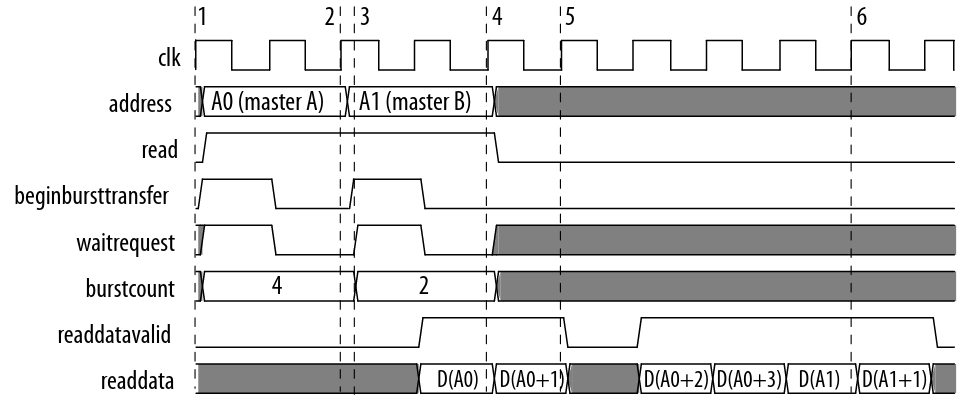
\includegraphics[width=12cm]{"res/chapter1/avalon_mm_read.png"}
  \caption{Read burst operation using Avalon MM}
  \label{fig:avalon_mm_read}
\end{figure}

\subsubsection{Write burst operation}

For writing, it's even simpler. As can be seen in Figure \ref{fig:avalon_mm_write}, the beginning will be similar to reading. The master will have to provide the first address, the length of the burst as well as pass the write and beginbursttransfer to high. In addition to that, the first word is also provided. Here again, the slave will respond with a waitrequest. As soon as the waitrequest is passed, the master will set the beginbusttransfer to low and send the words one after the other, starting at the next clock cycle. If the write signal goes down, the burst is paused and resumes as soon as it goes up again.

\begin{figure}[ht!]
  \center
  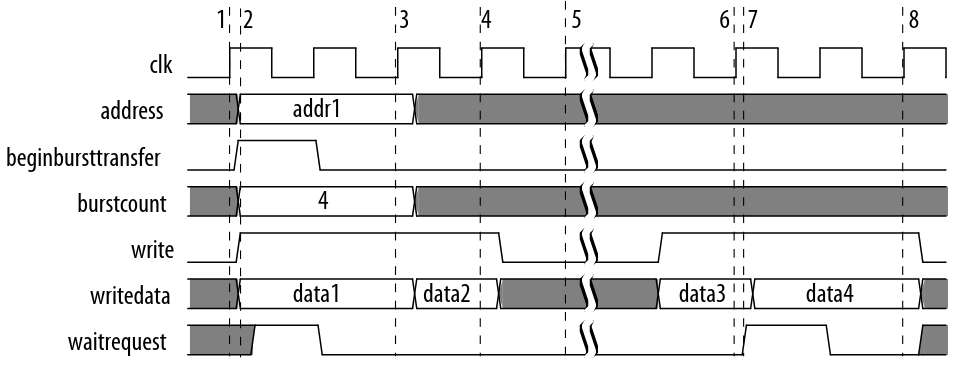
\includegraphics[width=12cm]{"res/chapter1/avalon_mm_write.png"}
  \caption{Write burst operation using Avalon MM}
  \label{fig:avalon_mm_write}
\end{figure}

\subsubsection{Inherent delays in communication}

In the end, communicating is not very complicated. However, the whole architecture using the bridges and this protocol must be able to manage delays and be adapted to them so that they do not degrade the efficiency of the machine too much. In these delays, it is necessary on the one hand to take into account the delays of the slaves, as well as the delays induced by the bursts if they are used. Cache and other solutions of the kind are to be studied in order to accelerate as much as possible the operations related to the communications between the two parts of the chip when it is possible.

\section{Getting hands: first implementations}

In this section two projects are described, one only using the FPGA side of the chip and the other one using the two sides. The reason for these first sub-projects is to verify the workflow of this
FPGA+SoC chip and to start working on it without having to directly confront a heavy and complete architecture. In addition, these two sub-projects consist of the realization of blocks that will be needed later on anyway. So nothing is lost.

\subsection{Using the FPGA side only: 8 bits counter with LEDs}

To check the development chain of this FPGA, an 8-bit counter has been implemented. This can be described very simply in verilog. As input this module takes the FPGA clock which oscillates at 50MHz and outputs the number contained in the 8-bit counter. The 8 bits are then mapped to the 8 LEDs on the board to make the number visible. However, with this update frequency, it is impossible to distinguish different numbers at the LEDs. The counter update frequency must therefore be reduced. An input is then added to the counter, the clock enable that will warn it when it needs to increment its value. To generate the clock enable, another module is implemented: the clock manager. This module is a counter that runs directly on the 50MHz except that it never returns its number. It will only count until it reaches a certain number that allows tuning the output frequency. In fact, as soon as the number is reached, the counter is reset to 0 and the clock enable goes to 1 for one clock tick. If the maximum number of the counter is set to $50 \times 10^6$, the clock enable will be generated once a second and the counter linked to the LEDs will be updated once a second as well. This makes reading at the LED level possible. The commented Quartus\footnote{Quartus Prime Lite 20.1 to be exact.} project of this subsection is available in \textsc{quartus/simple\_counter}.

\subsection{Using both the FPGA and the ARM sides}

Now that a counter has been created, the idea will be to access the DDR3 RAM on the ARM side from the FPGA side. To do this, the bridges and the avalon bus must be handled. The goal is to put a number at startup in the RAM (this is done on the ARM side), get it from the FPGA part, load it into the counter and start counting from there. Finally, the count has to be updated in RAM by the FPGA. Doing this ensures that the communication between the two parts of the chip, in both directions, works.

\vspace{12pt}
TO BE COMPLETED AS SOON AS IT IS DONE

\end{document}
